\documentclass{standalone}
\usepackage[T1]{fontenc}
\usepackage[final]{microtype}
\usepackage[english]{babel}
\usepackage{xcolor}
\usepackage{tikz}
\usetikzlibrary{calc}
\usepackage{fontspec}
\usepackage{sourcesanspro}
\setmainfont{STIXTwoText}[
  Extension={.otf},
  Path={./fonts/},
  UprightFont={*-Regular},
  BoldFont={*-Bold},
  ItalicFont={*-Italic},
  BoldItalicFont={*-BoldItalic}]
\setmonofont{CourierPrime}[
  Extension={.ttf},
  Path={./fonts/},
  UprightFont={*-Regular},
  BoldFont={*-Bold},
  ItalicFont={*-Italic},
  BoldItalicFont={*-BoldItalic},
  Scale=0.9]
\begin{document}
\begin{tikzpicture}
  % a rectangle with width (2 * 14 + 0.5 + 1.4 + 1.33) cm and height (21 + 0.5) cm
  \fill[white] (0,0) rectangle (31.23, 22.5);

  \node[anchor=south east, inner sep=0mm, line width=0mm] (image) at (31.23, 0) {%
    \reflectbox{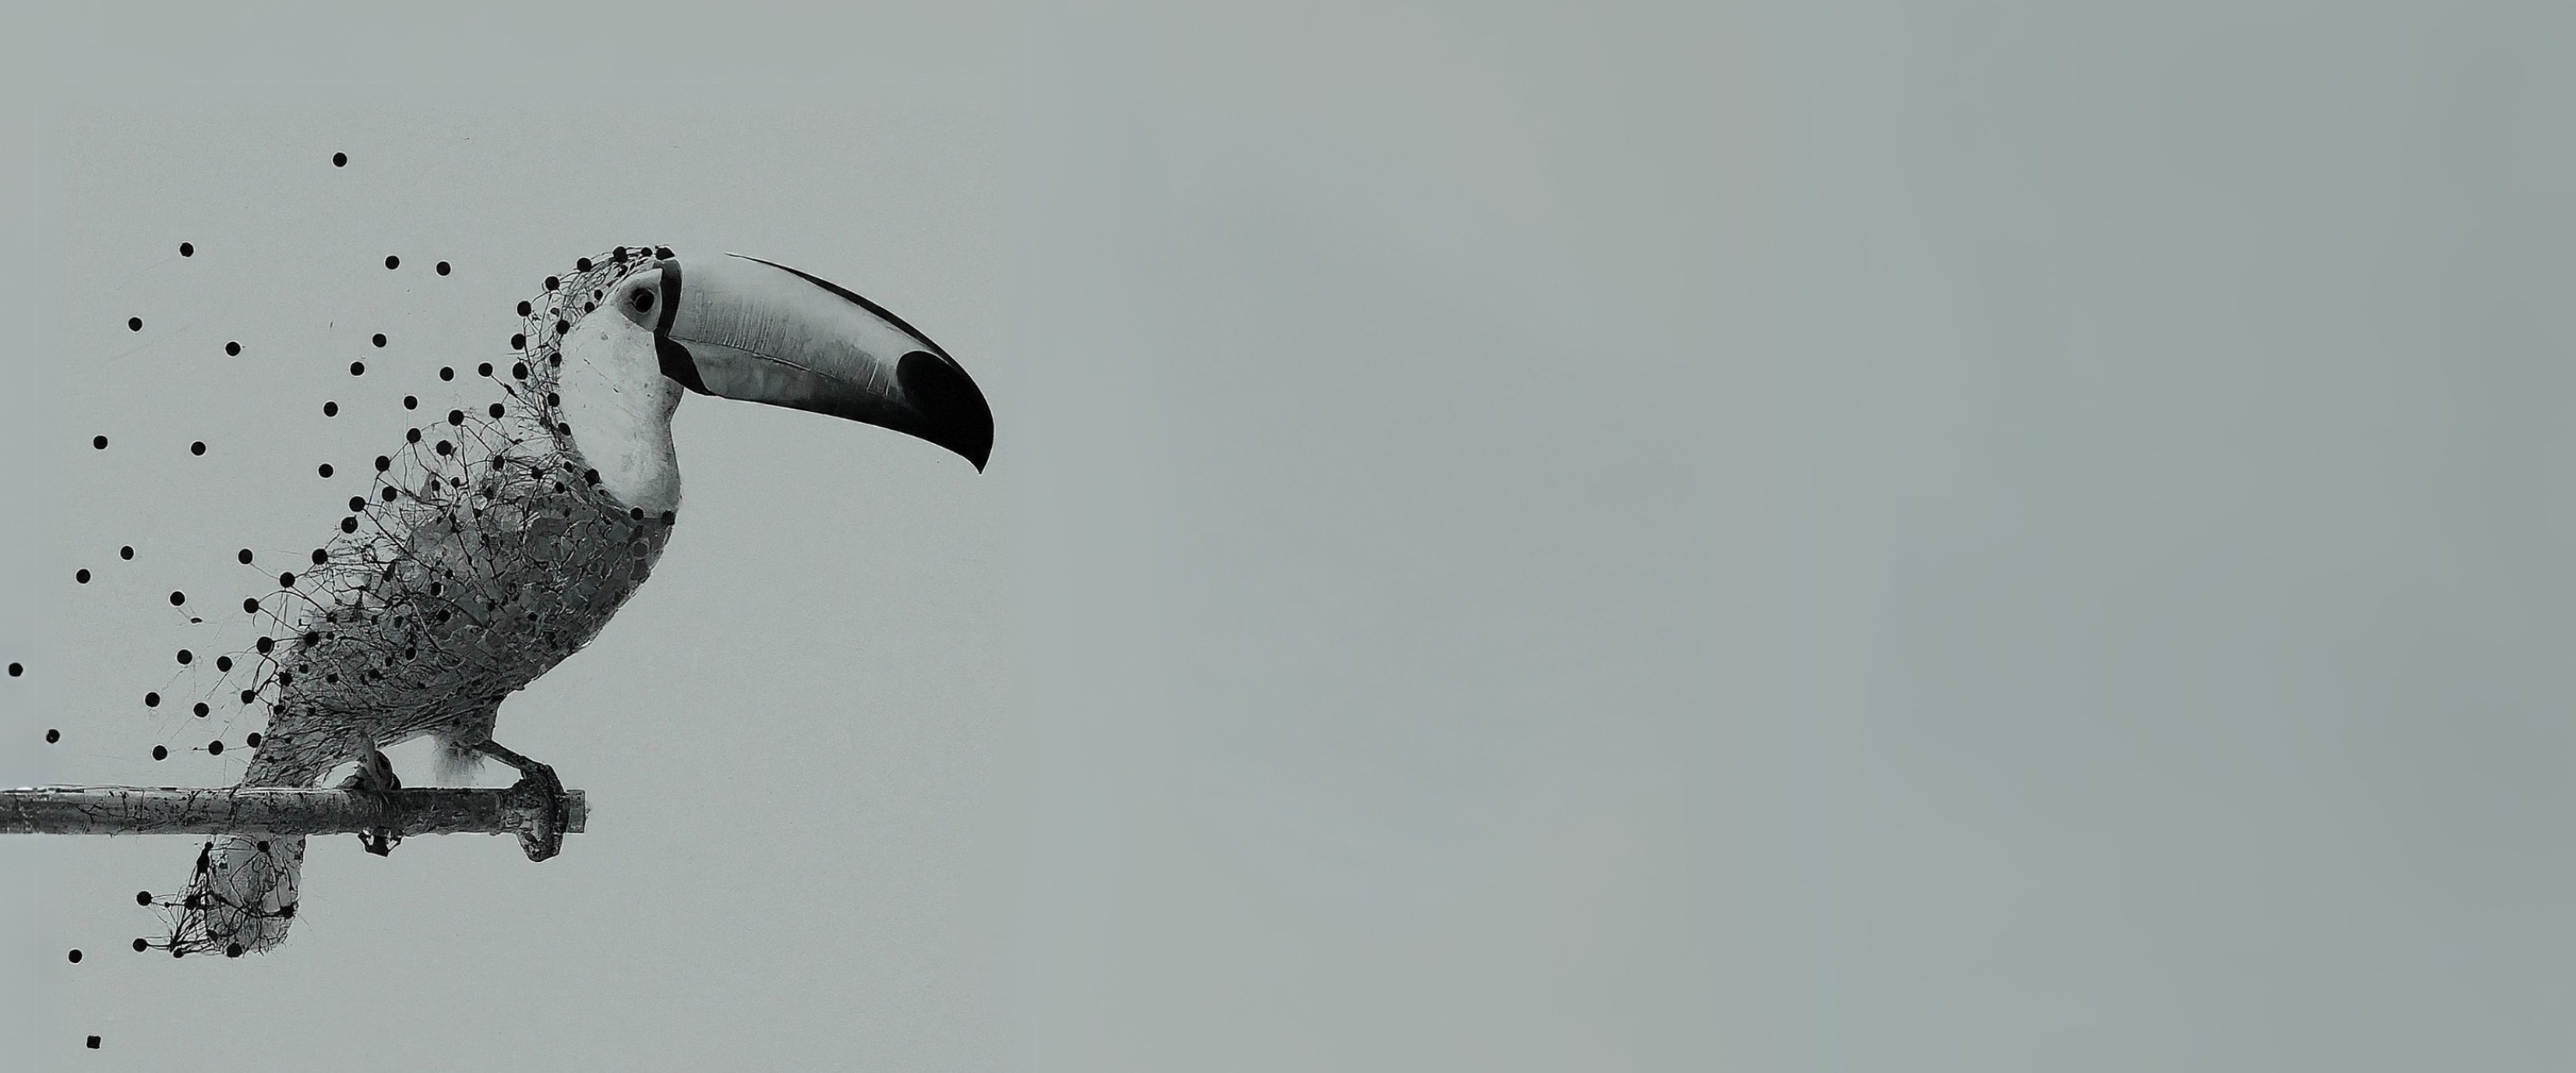
\includegraphics[width=31.23cm]{images/cover.jpg}}%
  };
  \fill[black!80] (image.north east) rectangle (0, 22.5);
  \node[white, anchor=center] (title) at (23.98, 17.75) {\Huge\sffamily\uppercase{Data Science Project}};
  \node[white,anchor=north, inner sep=5mm] at (title.south) {\LARGE\sffamily\uppercase{An Inductive Learning Approach}};
  \node[anchor=south west] at (18, 1) {\Huge\sffamily\uppercase{F.A.N. Verri}};

  % a white line with 1mm from image.north west to image.north east
  \draw[white, line width=1mm, yshift=0.5mm] ($(image.north west) + (0.05, 0)$) -- ($(image.north east) - (0.05, 0)$);

  \node[anchor=center, text width=12cm, align=center] at (7.25, 7.5) {%
    Filipe Verri is a Christian, happily married to Nayara Verri, and father of two boys.
    He holds a Computer Science degree (Hons.) from the University of São Paulo (USP) and
    a Ph.D.  in Computational Mathematics and Computer Science (Hons.) from the same
    institution.  During his Ph.D., he conducted a research internship at Arizona State
    University and received an Honorable Mention at the 8th USP Thesis Award in the major
    area of Earth and Exact Sciences.  From 2018 to 2024, he was an Assistant Professor at
    the Aeronautics Institute of Technology (ITA), where he coordinated strategic R\&D
    projects for the Brazilian Air Force in areas such as autonomous navigation,
    air traffic control, computer vision, and search and rescue. Currently, he works as an
    R\&D Consultant and is an Affiliate Professor at ITA and the Federal University of São
    Paulo (UNIFESP). His research focuses on Data Science, with an emphasis on Artificial
    Intelligence, Machine Learning, Complex Networks, and Complex Systems.
  };

  \node[anchor=center, text width=12cm, align=center, color=white] at (7.25, 17.25) {%
    ``Data Science Project: An Inductive Learning Approach'' provides a comprehensive
    methodology for data science project development, emphasizing software engineering
    principles essential for reliable solutions. Filipe Verri, a senior data science
    project manager, guides readers through the origins, scope, and key concepts of data
    science. This book covers machine learning, data handling, and rigorous validation
    techniques, all essential for preparing readers to tackle complex, real-world
    projects.
  };

  \node[anchor=center] (sponsor) at (7.25, 2.5) {
\includegraphics[height=1.5cm]{images/zippi.pdf}};
  \node[anchor=south] at (sponsor.north) {\sffamily This physical copy is offered to you by};
  \node[anchor=north] at (sponsor.south) {\sffamily zippi.com.br};

  \node[anchor=center, rotate=270] at (image.center) {%
    \large\sffamily\uppercase{Data Science Project: An Inductive Learning Approach}};

  \node[anchor=center, rotate=270, color=white] at (15.61, 17.25) {%
    \large\sffamily\uppercase{Filipe~\,A.~N.~\,Verri}};

  \path let \p1 = (image.north) in coordinate (mid) at (7.25, \y1);

  \node[circle, fill=white, anchor=center, minimum width=4cm] (photo) at (mid) {};
  \begin{scope}
    \clip (photo) circle (1.9cm);
    \node at (photo) {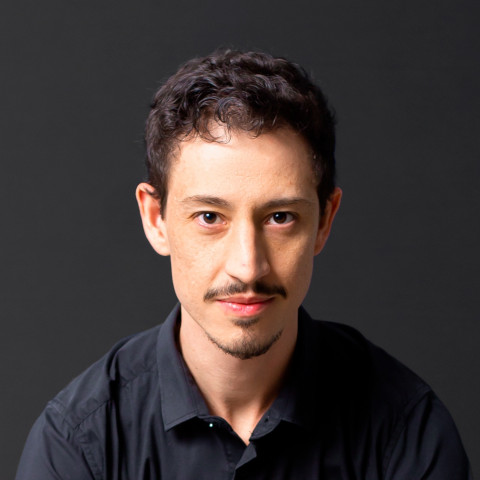
\includegraphics[width=4cm]{images/verri.jpg}};
  \end{scope}

  % \draw[dashed, black] (0.25, 0.25) rectangle (14.25, 21.25);
  % \draw[dashed, black] (14.25, 0.25) rectangle (14.95, 21.25);
  % \draw[dashed, black] (14.95, 0.25) rectangle (16.28, 21.25);
  % \draw[dashed, black] (16.28, 0.25) rectangle (16.98, 21.25);
  % \draw[dashed, black] (16.98, 0.25) rectangle (30.98, 21.25);
\end{tikzpicture}
\end{document}
